\section{Interactions}\label{interactions}

\begin{quote}
\begin{quote}
TODO: add tap options, how to draw, and a description of the tool-based
interface in general
\end{quote}
\end{quote}

\subsection{Tutorial}\label{tutorial}

We eschewed detailed drawing instructions or a separate tutorial mode,
in favor of short video tutorials that appear the first time each tool
is used. These tutorials can also be accessed by tapping the feature
icons on the about page.

\begin{figure}[htbp]
\centering
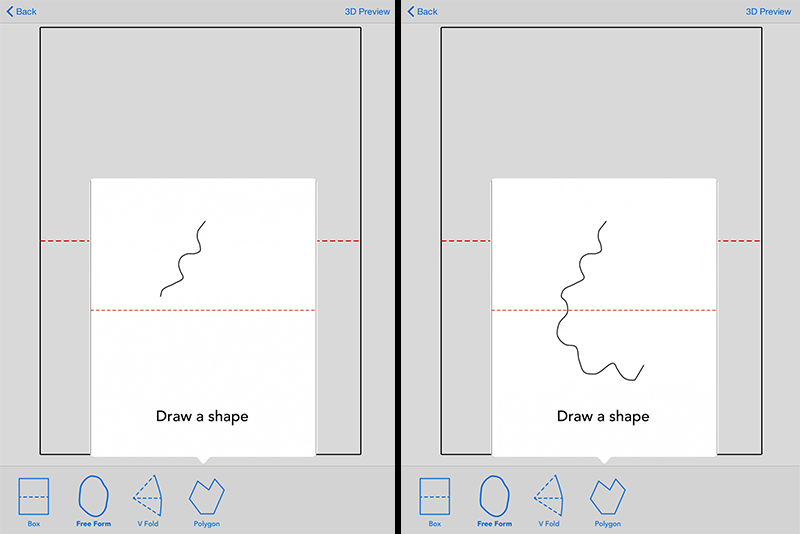
\includegraphics{figures/32_UI_Tool_Interactions/tutorial_step_one_two.png}
\caption{Free-form shape tutorial video.}
\end{figure}

We also show helpful tips between screens --- for example, when moving
to 3D preview and restoring from a saved sketch.

\subsection{Tool Interactions}\label{tool-interactions}

Some interactions are common to all features. To add a feature

\subsubsection{Box Fold}\label{box-fold}

To draw a

\subsubsection{FreeForm}\label{freeform}

\subsubsection{Polygon}\label{polygon}

\subsubsection{V-Fold}\label{v-fold}

\subsection{Warnings and Errors}\label{warnings-and-errors}

A central . We display warnings and error as

\begin{figure}[htbp]
\centering
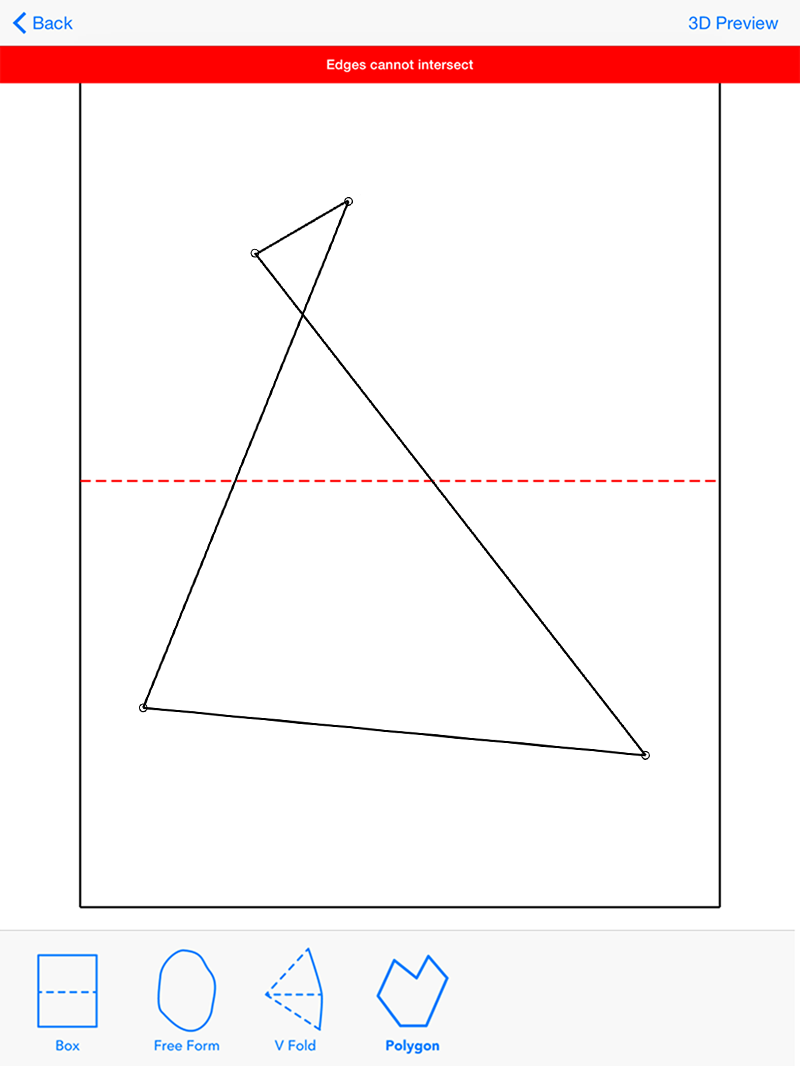
\includegraphics{figures/32_UI_Tool_Interactions/error_message.png}
\caption{An error message shown when rejecting a polygon with
intersecting edges.}
\end{figure}

\subsection{Send to Laser Cutter}\label{send-to-laser-cutter}

In the three-dimensional preview,

\subsection{Print}\label{print}

\begin{figure}[htbp]
\centering
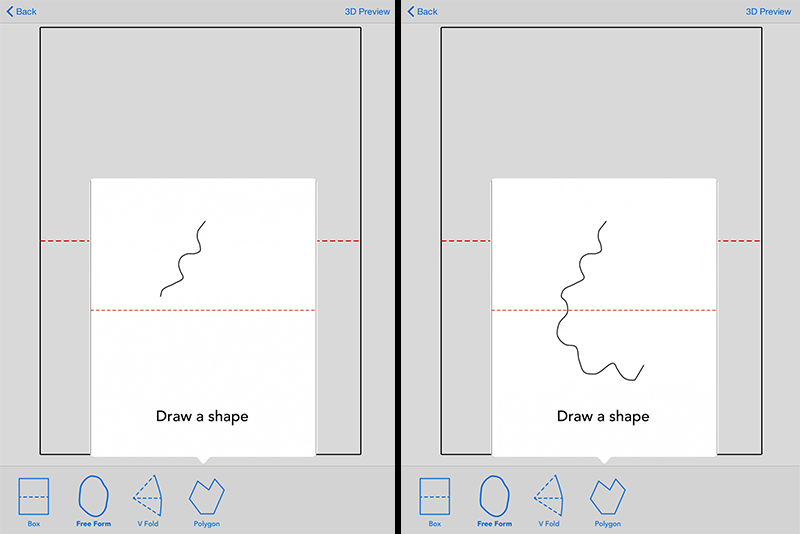
\includegraphics{figures/32_UI_Tool_Interactions/tutorial_step_one_two.png}
\caption{Options for sharing a fold pattern from the 3D preview.}
\end{figure}
